% Section 3.6: Dual Ensemble Architecture
\clearpage
\section{3.6 Dual Ensemble Architecture}
\label{sec:dual-ensemble}
\addcontentsline{toc}{section}{3.6 Dual Ensemble Architecture}

\lettrine{T}{he} Dual Ensemble Architecture provides two distinct execution environments optimized for different performance and safety requirements. This dual-layer approach enables ultra-low-latency execution for trusted operations while maintaining robust isolation for community-developed extensions.

\subsection*{3.6.1 The Pit: In-Process Execution}

The Pit constitutes the high-performance in-process execution environment for trusted infrastructure extensions. Five core components operate within The Pit: Pool Manager, DAG Tracker, Artifact Store, Arbitration Engine, and Stale Manager. Extensions execute within the same process as the core system, enabling direct function calls and shared memory access with nanosecond-level latencies.

\textbf{Institutional Memory and Resource Management Components}

The first architectural view of The Pit focuses on institutional memory, lifecycle management, and resource arbitration capabilities. As illustrated in Figure~\ref{fig:pit-core-memory-arbitration}, the PitCore serves as the central registry managing all in-process extensions through registration, unregistration, and retrieval operations. The PitCore maintains references to five critical infrastructure components, with three highlighted in this view.

The ArtifactStore provides Symphony's institutional memory system, storing artifacts with content-addressable hashing and Tantivy-based full-text indexing. Each artifact contains versioned data, metadata, quality scores, and timestamps, enabling efficient retrieval, search, and deduplication. The quality scoring mechanism ensures high-value artifacts receive priority in storage and retrieval operations.

The StaleManager handles artifact lifecycle transitions across storage tiers based on access patterns and age. The lifecycle management system defines three stages: SSD storage for frequently accessed artifacts (1-7 days), HDD storage for moderately accessed content (8-30 days), and cloud archival for long-term retention (30+ days). The StaleManager monitors artifact usage, triggers transitions between lifecycle stages, and performs cleanup operations to optimize storage utilization.

The ArbitrationEngine resolves resource conflicts when multiple workflows compete for limited resources. The engine maintains fairness policies, resolves conflicts through intelligent resource allocation strategies, applies fairness algorithms to prevent resource starvation, and prioritizes tasks based on urgency, importance, and historical patterns. This ensures optimal resource utilization while maintaining system responsiveness.

\begin{figure}[H]
\centering
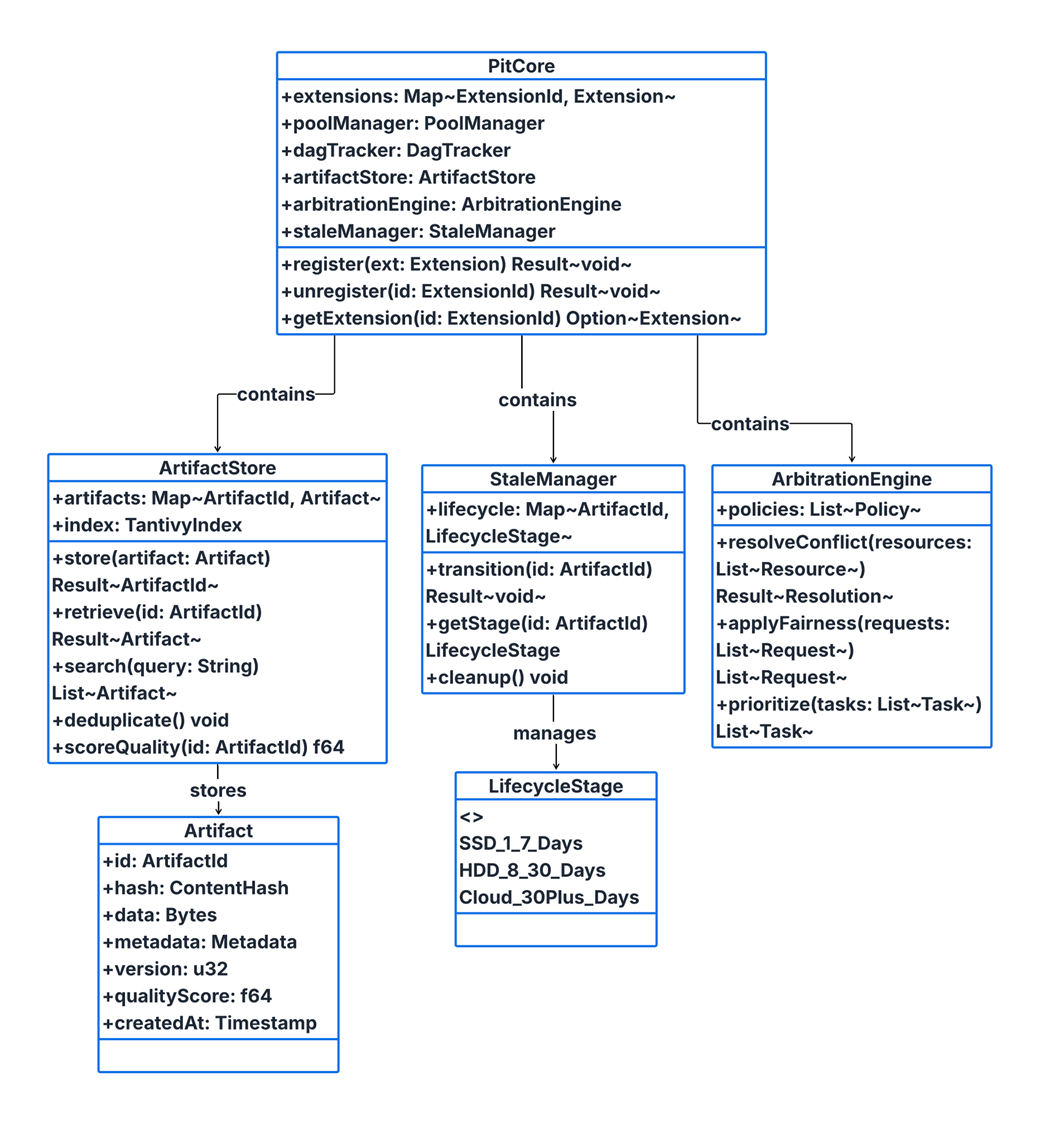
\includegraphics[width=1.0\textwidth]{images/diagrams/class_diagram/PitCore/PitCore1.png}
\caption{The Pit Architecture - Institutional Memory and Resource Management Components}
\label{fig:pit-core-memory-arbitration}
\end{figure}

\clearpage
\textbf{Workflow Execution and AI Model Management Components}

The second architectural view, shown in Figure~\ref{fig:pit-core-workflow-pool}, illustrates The Pit's workflow orchestration and AI model lifecycle management capabilities. The PitCore continues to serve as the central coordination point, now highlighting the DagTracker and PoolManager components that enable intelligent workflow execution and model resource optimization.

The DagTracker manages workflow execution through directed acyclic graph (DAG) representation and coordination. The tracker maintains a registry of workflows mapped by MelodyId, executes melodies by coordinating node execution according to dependency constraints, performs topological sorting to determine optimal execution order, supports parallel execution of independent nodes to maximize throughput, and provides checkpoint and resume capabilities for long-running workflows. Each DAG node represents a workflow step with defined inputs, outputs, extension identifiers, and parameter configurations.

The PoolManager handles AI model lifecycle management with intelligent resource optimization. The manager maintains a registry of players (AI models and extensions) mapped by ExtensionId, tracking their current state through the PlayerState enumeration (Unloaded, Loading, Warming, Ready, Active). The LRU cache mechanism optimizes memory utilization by tracking recently used models and evicting least-recently-used entries when memory pressure increases. The predictive pre-warming capability analyzes usage patterns to anticipate which models will be needed next, proactively loading them before requests arrive to minimize perceived latency. The allocation and deallocation methods manage player lifecycle, while state queries enable the system to make informed scheduling decisions.

Together, these components enable The Pit to achieve microsecond-level operation latencies through in-process execution, shared memory access, and zero-copy data transfer between components. This performance profile makes The Pit essential for Symphony's real-time AI orchestration and workflow execution capabilities.

\begin{figure}[H]
\centering
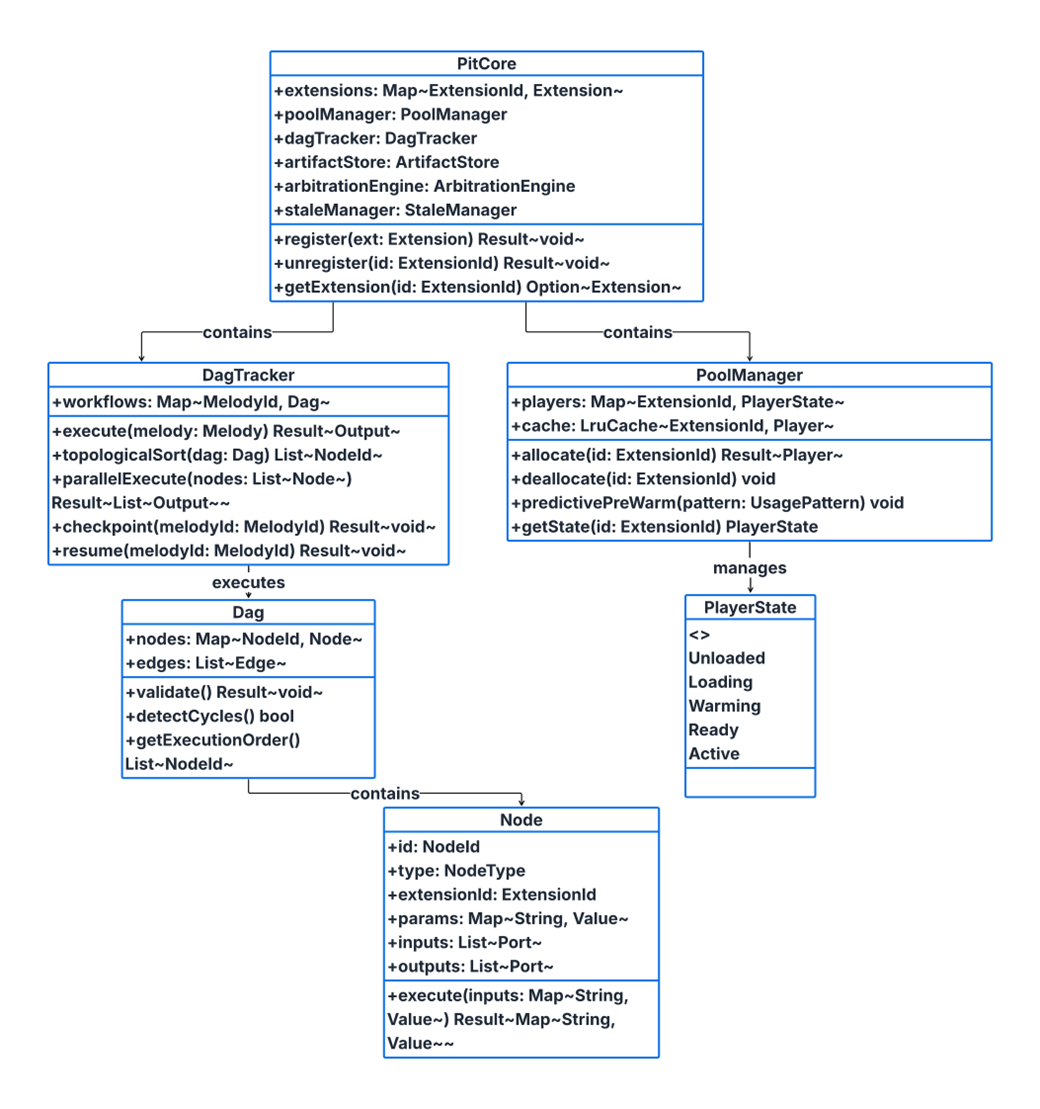
\includegraphics[width=1.0\textwidth]{images/diagrams/class_diagram/PitCore/PitCore2.png}
\caption{The Pit Architecture - Workflow Execution and AI Model Management Components}
\label{fig:pit-core-workflow-pool}
\end{figure}

\clearpage
\subsection*{3.6.2 The Grand Stage: Out-of-Process Execution}

The Grand Stage provides the out-of-process execution environment for community-developed extensions requiring strong isolation guarantees. Extensions execute in separate processes with well-defined communication channels, ensuring that bugs or malicious behavior cannot compromise system stability or security. The Grand Stage employs an actor-based concurrency model where each extension runs as an independent actor with its own mailbox for receiving messages.

While The Grand Stage incurs additional overhead from inter-process communication resulting in latencies measured in fractions of a millisecond, this overhead remains imperceptible to users for most operations and provides essential protection against risks of running untrusted code.

\subsection*{3.6.3 Security and Trust Framework}

Symphony implements a multi-layered security approach protecting users while enabling innovation as shown in ~\ref{Multi-Layer Security Framework}:

\begin{table}[H]
\caption{Multi-Layer Security Framework}
\label{Multi-Layer Security Framework}
\centering
\begin{tabular}{@{}lll@{}}
\toprule
\textbf{Security Layer} & \textbf{Mechanism} & \textbf{Protection} \\
\midrule
Sandboxed Execution & Process isolation & Fault containment \\
Permission System & Capability-based access & Resource protection \\
Code Review & Automated scanning & Vulnerability prevention \\
Runtime Monitoring & Behavioral analysis & Anomaly detection \\
\bottomrule
\end{tabular}
\end{table}

The capability-based security framework provides fine-grained control over extension permissions through minimal privilege principle, dynamic capability adjustment based on behavior and trust levels, capability inheritance for controlled privilege escalation, and immediate revocation mechanisms in response to security threats.

The trust-based security model adapts to extension behavior over time through behavioral trust scoring with continuous assessment of patterns, community trust metrics integrating user feedback and ratings, graduated trust levels providing progressive capability access based on demonstrated reliability, and trust decay mechanisms for inactive or problematic extensions.

\subsection*{3.6.4 Player Registration System}

Extensions can register as Players to participate in Conductor orchestration, gaining enhanced capabilities and visibility. The Player system provides:

\begin{compactlist}
    \item Intelligent extension selection based on workflow requirements
    \item Performance monitoring and quality assurance
    \item Enhanced integration with Symphony's AI orchestration
    \item Elevated marketplace visibility and user trust
\end{compactlist}

Players commit to governance policies including performance standards and security compliance, with continuous SLA monitoring ensuring adherence. The Conductor chooses optimal Players for tasks based on capabilities, performance characteristics, and trust levels.

\subsection*{3.6.5 Execution Strategy Selection}

The system determines execution environment based on multiple factors including trust level, performance requirements, resource usage patterns, and security considerations. Infrastructure extensions that are part of Symphony's core distribution execute in The Pit for optimal performance, while community-developed extensions and experimental features execute on The Grand Stage for isolation and protection.
